\documentclass[class=article, crop=false]{standalone}
\usepackage[subpreambles=true]{standalone}

\usepackage{preamble}

\begin{document}



% \begin{wrapfigure}{i}{\textwidth}
\begin{center}
    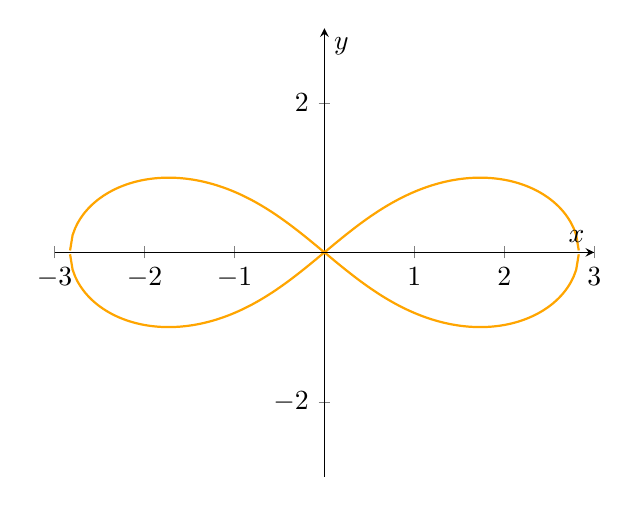
\begin{tikzpicture}
    \begin{axis}[
        xlabel=$x$,
        ylabel={$y$},
        domain=-3:3,
        samples=200,
        axis lines=middle,
        ymin=-3,
        ymax=3
    ]
    \addplot[thick, color=Orange, domain=-2.828:2.828]{sqrt(4*sqrt(1+x^2)-x^2-4)};
    \addplot[thick, color=Orange, domain=-2.828:2.828]{-sqrt(4*sqrt(1+x^2)-x^2-4)};
    \addplot[]{0}; % я добавил эту штуку, чтобы показать небольшие пустые поля (domain=-3:3), но это нехорошо. надо пофиксить
    \end{axis}
    \end{tikzpicture}
    
    \caption{Лемниската Бернулли}
    \label{fig:task2}
\end{center}
% \end{wrapfigure}

Выполненная работа в Desmos доступна по 
\href{https://www.desmos.com/calculator/23qokppxuf?lang=ru}{ссылке}

\subsubsection*{Ход работы}

\begin{enumerate}
    \item На графике с полярными координатами изобразили лемнискату Бернулли.
    
    \item Формула для нахождения интеграла в полярных координатах:
    $$
    S\ =\ \frac{1}{2}\int\limits_{\phi_{1}}^{\phi_{2}}\rho^{2}\left(\phi\right)d\phi$$
    
    \item Вычислим данный интеграл:
    $$
    S\ =4\cdot\ \frac{1}{2}\int\limits_{0}^{\frac{\pi}{4}}8\cos2\theta\ d\theta\ =\ 8\cdot\left(\sin\left(2\cdot\frac{\pi}{4}\right)-\sin\left(2\cdot0\right)\right)=8
    $$
        Интеграл брался от 0 до $\frac{\pi}{4}$, так как период функции $\cos2\theta$ это $\pi$, следовательно четвертью является $\frac{\pi}{4}$. В свою очередь, четверть отрезка мы берём, так как лемниската симметрична относительно центра координат и оси $0Y$.

    
\end{enumerate}

\subsubsection*{Заключение}

Правдоподобность рассчитанной площади можно оценить, взглянув на график лемнискаты в координатах $X0Y$. Видно, что график ограничен прямоугольником размером 6 на 2. Рассмотрим первую четверть. В ней, на графике отмечены два треугольника, общей площадью равной 1. Для оценки вычтем данную площадь, умноженную на 4, из площади прямоугольника. Мы умножали площадь треугольников на 4, так как лемниската симметрична, относительно начала координат и оси $0Y$, а значит график идентичен во всех четвертях. Итого, получаем оценочную площадь равной 8. Так как сам интеграл оказался так же равен 8, то можем считать, что вычисления точны.

\newpage

\end{document}